%!TEX root = ../../../adrien_gomar_phd.tex
\chapter{Contra-rotating open rotors}
\label{cha:cror}

\chabstract{In this chapter, we first recall the thrust
and propulsive efficiency equations. Using them,
the propeller engines are shown to be good candidates
for efficient alternative engines, mainly due to a high bypass ratio.
Geometry, general principles, similarity coefficients
and main physical phenomena of such engines are 
described. In addition to that, it is shown that even if efficient,
propeller engines suffer from a residual swirl motion.
To tackle this problem, the contra-rotating open rotor
technology is presented along with its main source of unsteadiness.
The challenges associated to this engine are finally detailed
and we show that aeroelasticity needs to be accounted for.}


\newpage

\section{Generalities of propulsion}
\label{sec:cror_intro}
%!TEX root = ../../../adrien_gomar_phd.tex

For an aircraft in steady flight conditions, 
lift balances weight and 
thrust balances drag. This explains why engineers try
indefinitely to reduce weight while increasing
thrust. A trade-off between both aspects is to work
on the propulsive efficiency of the engine. In this
section, general information on propulsion are given,
that leads to the concepts of propeller and
contra-rotating open rotor.

\subsection{Thrust equation}
\label{sub:cror_thrust}

The force applied on an engine, namely the thrust,
comes from the static pressure
distribution and the viscosity of the wetted areas.
To compute it, we assume for simplicity that:
 \begin{itemize} \itemsep0pt \parskip0pt
  \item the engine is schematically represented by a tube,
  as shown in Figure~\ref{fig:engine_parametrization},
  \item the flow is steady (steady-state hypothesis),
  \item the viscosity effects are negligible compared
  to the pressure effects,
  \item the pressure surrounding the engine $p_\infty$
  is constant,
  \item the inlet pressure $p_0$, the outlet pressure
  $p_1$ and the pressure surrounding the engine $p_\infty$ are equal,
  meaning that the nozzle is adapted.
\end{itemize}
The problem parametrization is schematically represented
in Figure~\ref{fig:engine_parametrization}.
\begin{figure}[htp]
  \centering
  \subfigure{
      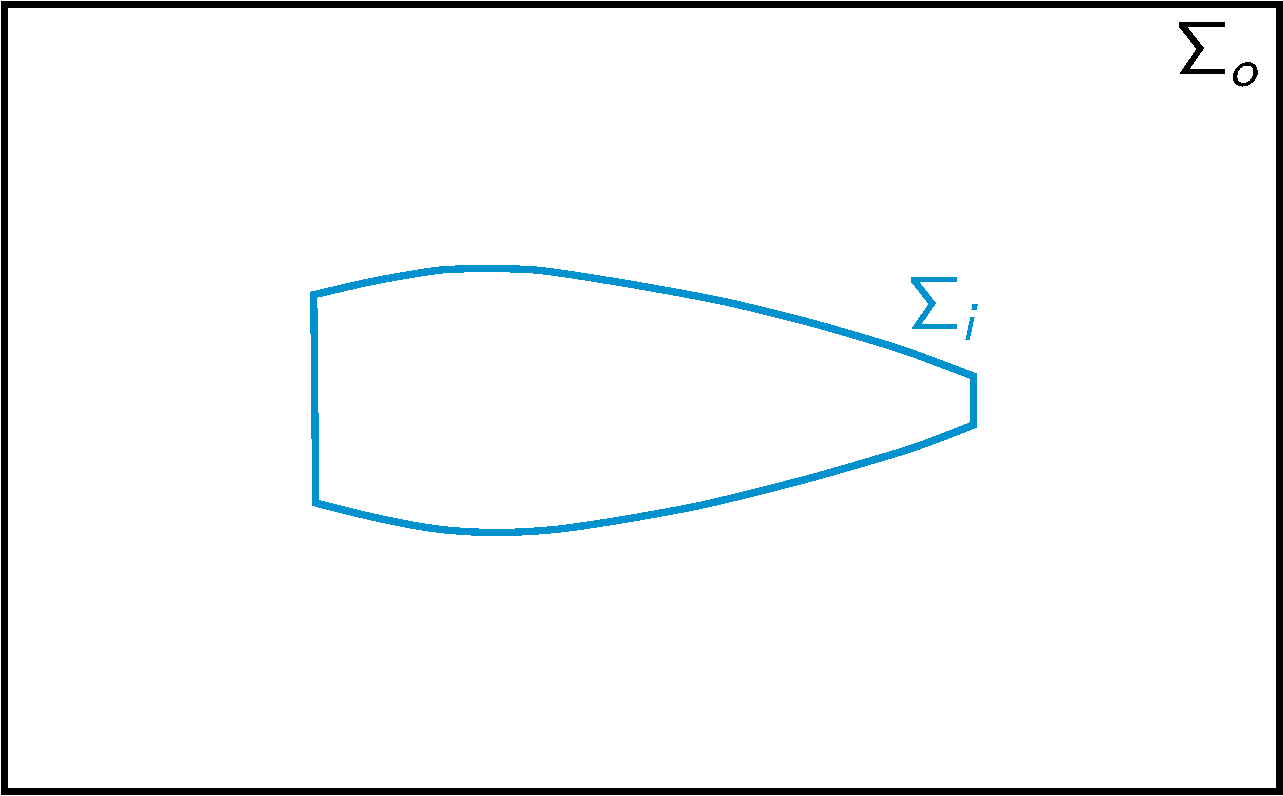
\includegraphics[scale=.3]{control_volume.pdf}}
  \quad\subfigure{
      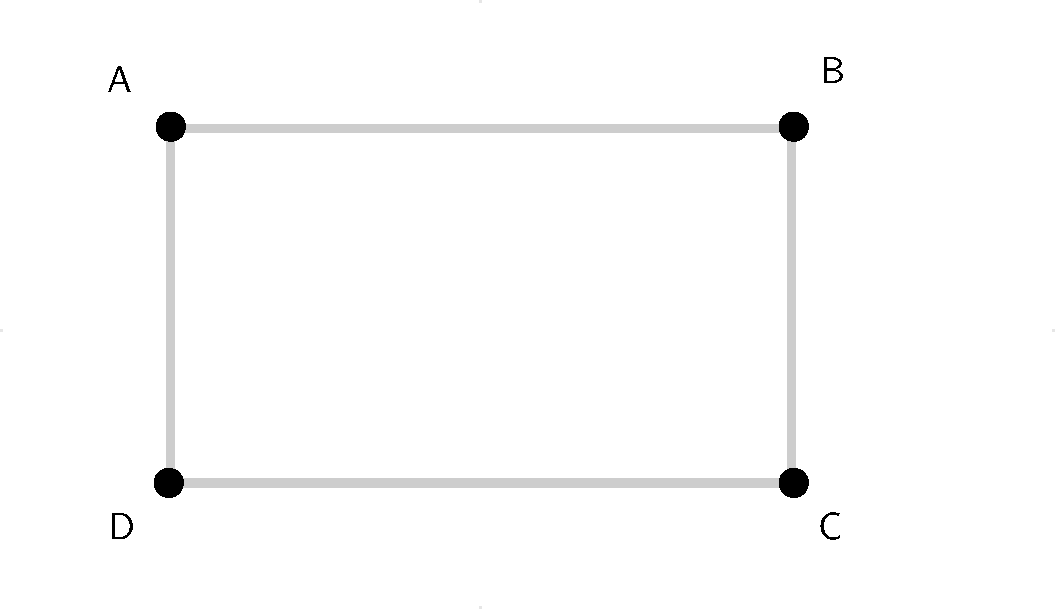
\includegraphics[scale=.3]{control_volume_2.pdf}}
  \caption{Engine parametrization for the computation of the thrust.}
  \label{fig:engine_parametrization}
\end{figure}
With the given hypothesis, the thrust, which is
the resultant force
projected onto the x-axis, is defined as
\begin{equation}
	F_x = \iint_{BC + DA} p_{int} \diff \vec{S} - 
	    \iint_{BC + DA} p_{\infty} \diff \vec{S},
	\label{eq:thrust_1}
\end{equation}
where $p_{int}$ is the internal static
pressure distribution. The integral on
$AB + CD$ is zero due to the projection on
the x-axis.
Moreover, as the surrounding pressure is constant
\begin{equation}
	\iint_{BC + DA} p_{\infty} \diff \vec{S} =
	p_{\infty} \iint_{BC + DA} \diff \vec{S} =
	p_{\infty} (S_{1} - S_{0}).
	\label{eq:thrust_2}
\end{equation}
The distribution of internal pressure is
difficult to estimate. To alleviate this, 
we make use of the Euler’s momentum 
equation applied to the internal fluid
\begin{equation}
	\iint_{S} \left(\rho \vec{V} \cdot \diff \vec{S} \right) V = 
	\iint_{S} p \diff \vec{S}
	\label{eq:thrust_3}
\end{equation}
The velocity being zero at walls, 
the left-hand side of the Eq.~\eqref{eq:thrust_3}
simplifies to
\begin{equation}
	\iint_{S} \left(\rho \vec{V} \cdot \diff \vec{S} \right) V =
	- \rho_0 V_0 S_0 V_0 +  \rho_1 V_1 S_1 V_1 = 
	\dot{m} \left( V_{1} - V_{0} \right),
\end{equation}
where $\dot{m}$ is the mass-flow rate going through the engine.
The right-hand side of Eq.~\eqref{eq:thrust_3}, projected onto
the x-axis, is equal to 
\begin{equation}
	\iint_{S} p \diff \vec{S} = 
	\iint_{BC + DA} p \diff \vec{S} = 
	p_{\infty} \iint_{BC + DA} \diff \vec{S} =
	p_{\infty} (S_{1} - S_{0}),
\end{equation}
since we consider that $p_0 = p_1 = p_\infty$.
Finally the thrust $F_x$ simplifies to
\begin{equation}
	\fbox{$
	F_x = \dot{m} (V_{1} - V_{0})
	$}
	\label{eq:cror_thrust}
\end{equation}
From this simple equation,
one can see that to increase the thrust $F_x$, there are two parameters:
the mass-flow and the axial velocity increment.

\subsection{Global propulsive efficiency}
\label{sub:cror_efficiency}

The global propulsive efficiency $\eta$ measures the 
success in converting a mechanical power into a
propulsive power. It results from the combination
of the kinetic efficiency $\eta_{K}$ and the propulsive efficiency
$\eta_{PR}$
\begin{equation}
	\eta = \eta_{K} \times \eta_{PR}.
\end{equation}
This is schematically represented in Figure~\ref{fig:cror_efficiency}.
\begin{figure}[htp]
  \centering
  \includegraphics*[width=0.5\textwidth]{efficiency.pdf}
  \caption{Efficiency relations from mechanical power to propulsive power.}
  \label{fig:cror_efficiency}
\end{figure}

\paragraph{Kinetic efficiency}
The kinetic efficiency measures the success in converting the mechanical
power $P_m$ into a kinetic power $P_k$
\begin{equation}
	\eta_K = \frac{P_k}{P_m}.
\end{equation}

The mechanical power delivered as input
can be computed through the first thermodynamic principle. In fact, in absence
of heat exchange, the mechanical power $P_m$ can be estimated as
\begin{equation}
	P_m = \dot{m} (h_{i_{1}} - h_{i_{0}}),
\end{equation}
where $h_i$ is the total enthalpy and subscript $0$ and $1$ are
the input and output of the propulsion system, respectively, as represented
in Figure~\ref{fig:engine_parametrization}.
The kinetic power $P_k$ is given by
\begin{equation}
	P_k = \dot{m} \left(\frac{1}{2} V^2_{1} -
	\frac{1}{2} V^2_{0} \right).
\end{equation}
This leads to a kinetic efficiency that can be expressed as
\begin{equation}
	\eta_{K} = \frac{V^2_{1} - V^2_{0}}{2 (h_{i_{1}} - h_{i_{0}})}.
\end{equation}

\paragraph{Propulsive efficiency}
The propulsive efficiency $\eta_{PR}$ measures the success
in creating a propulsive power $P_{pr}$ from a
kinetic power $P_k$
\begin{equation}
	\eta_{PR} = \frac{P_{pr}}{P_k}.
\end{equation}
The propulsive power is computed using the thrust $F_x$
\begin{equation}
	P_{pr} = F_x \times V_{\infty},
\end{equation}
where $V_{\infty}$ is the free-stream velocity.
Finally, if the free-stream velocity is the inlet velocity $V_{0}$
and the inlet and outlet velocities are purely axial
\begin{equation}
	\fbox{$
	\eta_{PR} = \displaystyle \frac{1}{1 + \frac{V_{1} - V_{0}}{2 V_{0}}}
	$}
	\label{eq:cror_propulsive_efficiency}
\end{equation}
This formula means that the most efficient engine produces
a very small velocity increment.

\subsection{Toward propeller engines}
\label{sub:cror_toward_propeller}

One way to improve the environmental footprint of
airplanes engines is to increase the propulsive efficiency
by reducing the kinetic power needed to drive the engine.
According to the propulsive efficiency 
formula, doing so while maintaining the thrust can be achieved through
a higher mass-flow rate. Two new concepts are thus derived from
this simple statement: the
Ultra-High Bypass Ratio (UHBR) which
is basically a turbofan with a larger fan exhaust, and the
propeller, the mass-flow rate of which is not limited
by the architecture, as the blades are not within a nacelle.
In the following section, the propeller engine will be detailed
and the drawbacks of such an architecture will be highlighted to
motivate the use
of a second propeller row, yielding the contra-rotating open rotor
architecture.




\section{Propellers}
\label{sec:cror_propeller}
%!TEX root = ../../../adrien_gomar_phd.tex

\subsection{Geometry}
\label{sub:cror_propeller_geometry}

A propeller is composed of a hub and a rotating set of 
$B$ blades as schematically represented in
Figure~\ref{fig:cror_propeller_geometry}. The hub
is the part on which the blades are mounted.
We set the diameter of these blades being $D$
and their rotation speed being $\Omega$. 
In front of the propeller, there is a spinner which is
a conic element that conducts the 
inflow to the propeller blades.
The propeller can be seen as
a turbofan whose fan is not within a nacelle.
\begin{figure}[htp]
  \centering
  \includegraphics*[scale=0.30]{propeller_geometry.pdf}
  \caption{Geometry of a propeller.}
  \label{fig:cror_propeller_geometry}
\end{figure}
This absence implies that theoretically, the mass-flow can be
infinite. To quantify this, it is common for engines to
consider the bypass ratio. It is defined as the ratio of the
cold air (the fan exhaust)
divided by the hot air (the air that goes through the engine core).
To give an idea, one of the highest bypass ratio engine on today's aircraft is obtained
by the Pratt~\&~Whitney~PW1000G with a~12 bypass ratio. 
This number is representative of the mass-flow rate generated by the engine.
However, we have seen that mass-flow and the velocity
difference are the two parameters that can be used to increase
the thrust. Assuming that in a classical ducted turbofan, 
the bypass ratio is limited to~12, the only
way to further increase the thrust is to increase the 
velocity which deteriorates the propulsive efficiency.
For the sake of comparison, 
propellers are estimated to have a bypass ratio of~50. 
This explains why this architecture has
regained interest.

\subsection{Velocity triangle}
\label{sub:cror_propeller_velocity_triangle}
The velocity triangle applied to a propeller configuration
is shown in Figure~\ref{fig:cror_velocity_triangle_propeller}.
The aim of a propeller is to create thrust through an increase
of the axial velocity noted $\Delta V_x$ in the diagram. To do
so, the relative flow field is straighten up. This gives both
an increase in axial velocity but also in tangential velocity.
In fact, the inflow that was purely axial retrieves a tangential
component at the outlet. This is called the swirl and
is a lost energy as it cannot be used to produce thrust.
\begin{figure}[htp]
  \centering
  \includegraphics*[scale=0.55]{velocity_triangle_propeller.pdf}
  \caption{Velocity triangle applied to a propeller.}
  \label{fig:cror_velocity_triangle_propeller}
\end{figure}
Moreover, the relative velocity $W$ should be kept subsonic
otherwise the propulsive efficiency is reduced. This limits
the free-stream velocity $V_0$ of the aircraft and the size of 
the propeller as the rotation speed velocity depends on
the radius of the blades. This explains why propellers have
been limited so far to low-speed inflow conditions.

\subsection{Similarity coefficients}
\label{sub:similarity_coefficients}
To evaluate the performance of the propeller, four similarity
coefficients are commonly used:
the advance ratio $J$ that represents the operating point of the propeller,
the thrust $C_t$ and power $C_p$ coefficients and finally
the efficiency $\eta$
\begin{equation}
    J = \frac{V_0}{n D}, \quad
    C_T = \frac{F_x}{\rho n ^ 2  D ^ 4}, \quad
    C_P = \frac{M_x \Omega}{\rho n ^ 3 D ^ 5}, \quad
    \eta = J \frac{C_T}{C_P},
\end{equation}
where $V_0$ is the free-stream velocity 
as shown in Figure~\ref{fig:cror_propeller_geometry},
$\rho$ the free-stream density,
$n$ the rotation frequency ($n = \Omega / 2 \pi$),
$F_x$ the thrust and
$M_x$ the axial torque.
The efficiency defined here is actually the global propulsive efficiency
as it gives the ratio of the propulsive power over the mechanical power.

An estimation of the variation of the advance ratio $J$ and the 
efficiency $\eta$ depending on the flight conditions is 
given by~\citet{Bousquet2012}
\begin{alignat}{4}
    \text{(cruise)} \quad  0.8 &< \eta &< 0.95, \quad 1 &< J < 3.5 \\
    \text{(take-off and landing)} \quad  0.5 &< \eta &< 0.8, \quad J &< 1.
    \label{eq:estimation_sim_coeff}
\end{alignat}

\subsection{Main physical phenomena}
\label{sub:cror_propeller_physics}

The main physical phenomena that can be seen in a propeller are schematically represented
in Figure~\ref{fig:propeller_phys_phenomena}. 
\begin{figure}[htp]
  \centering
  \subfigure[wakes]{
      \label{fig:propeller_wakes}
      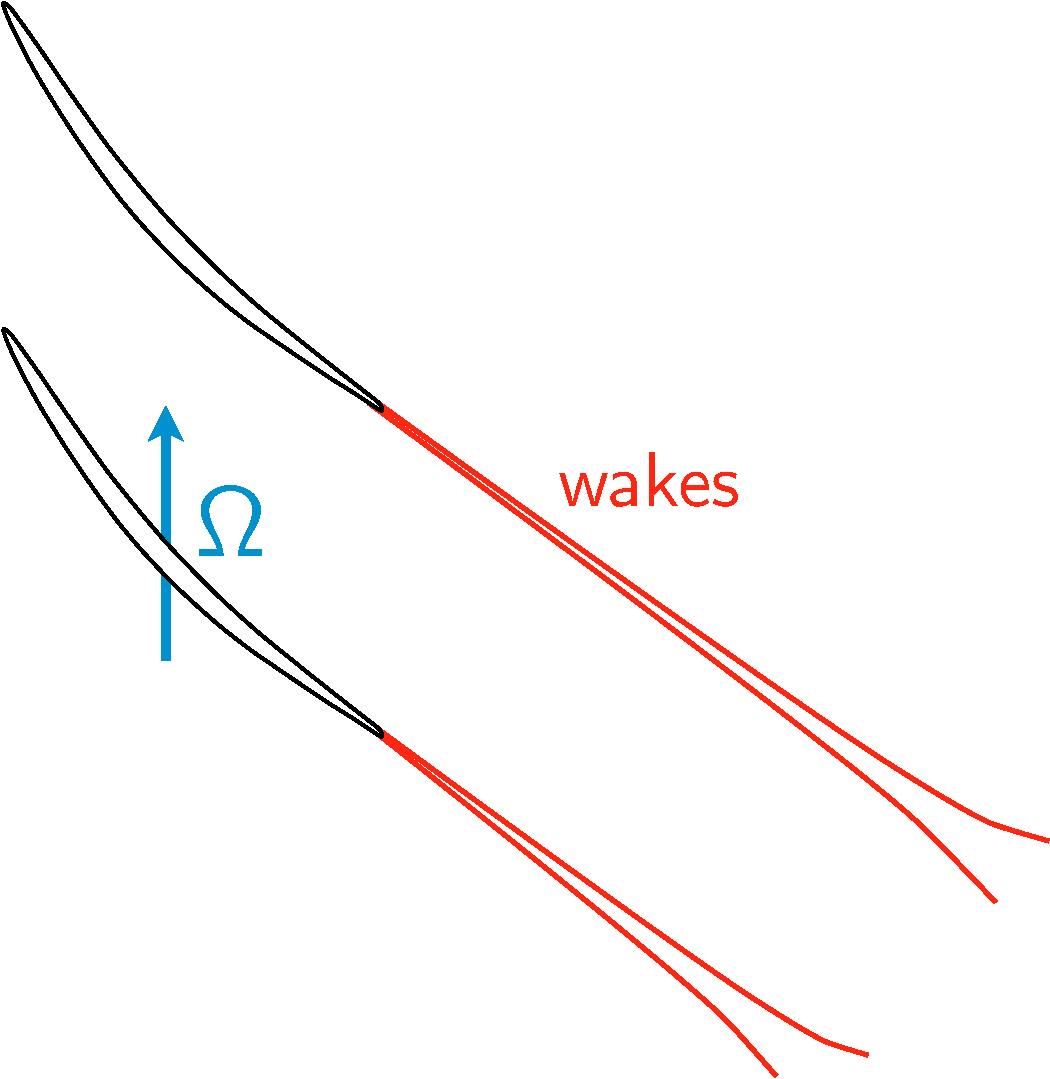
\includegraphics[scale=.2]{propeller_wakes.pdf}}
  \quad\subfigure[tip vortices]{
      \label{fig:propeller_tip_vortices}
      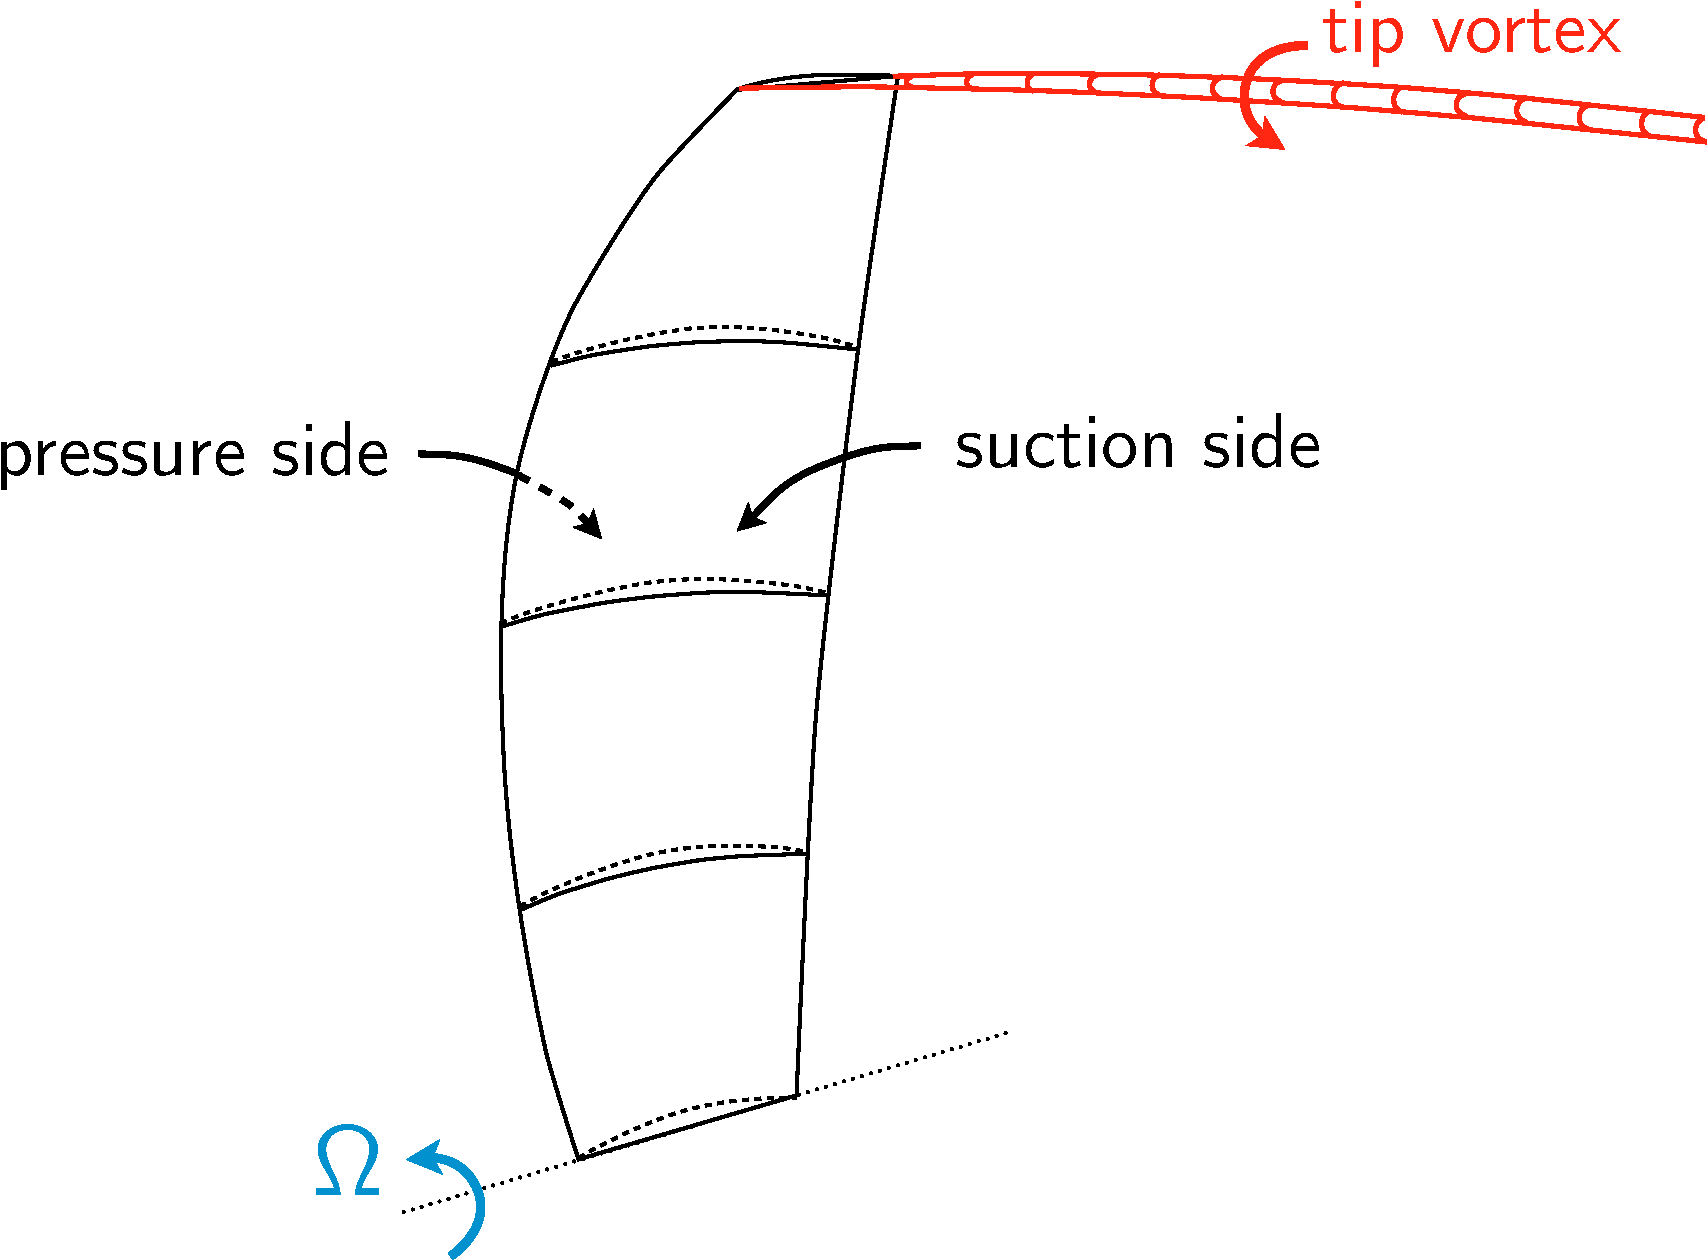
\includegraphics[scale=.2]{propeller_tip_vortices.pdf}}
  \quad\subfigure[stream tube contraction]{
      \label{fig:propeller_stream_tube}
      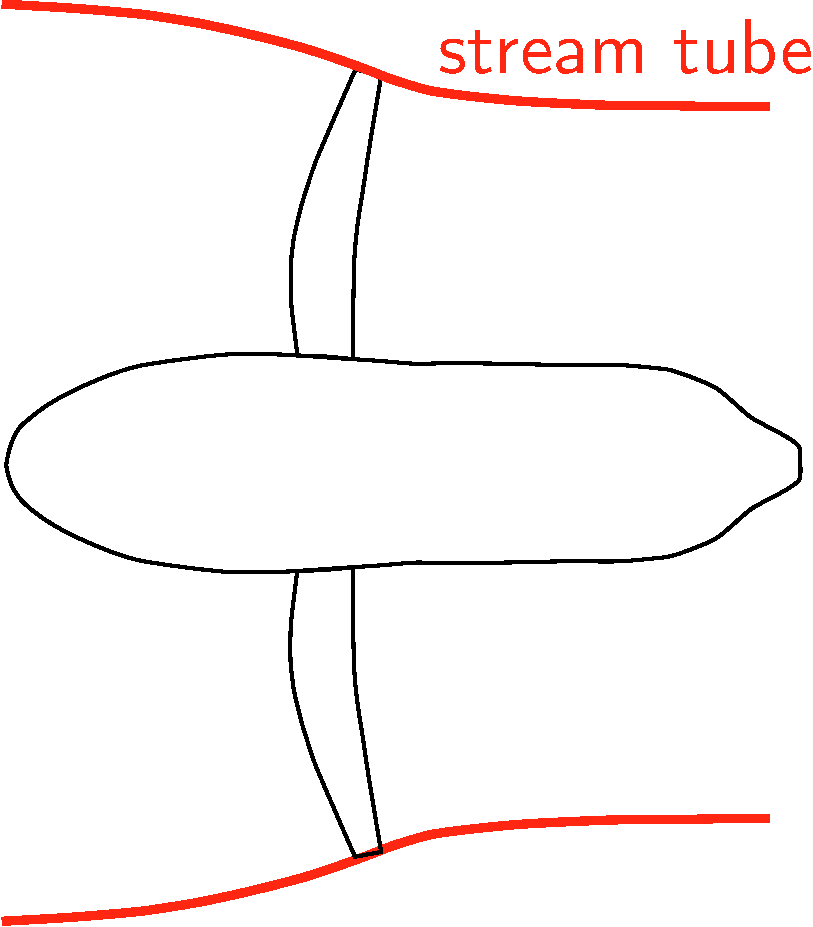
\includegraphics[scale=.2]{propeller_stream_tube.pdf}}
  \caption{Main physical phenomena seen in a propeller.}
  \label{fig:propeller_phys_phenomena}
\end{figure}
Firstly, due to the presence of a boundary
layer on the pressure and suction sides of the blades, a wake is shed behind each blade, which involves a momentum deficit (Figure~\ref{fig:propeller_wakes}). 
It is mostly a two-dimensional
phenomenon seen at each radius. Secondly, 
in the tip region of the blade, the pressure difference between each 
side of the blade induces a vortex that is counter-rotating with respect to 
the rotation speed (Figure~\ref{fig:propeller_tip_vortices}). 
They are advected by the local relative velocity giving them
an helical path propagating downstream.
To reduce this phenomenon, one way is to modify the geometry of the tip
of the blades.
Finally, the propeller generates thrust through an acceleration of the fluid. Thus, the stream
tube is contracted (Figure~\ref{fig:propeller_stream_tube}). 
All of these phenomena are stationary in their relative frame of reference.


\section{Contra-rotating open rotors}
\label{sec:cror_cror}
%!TEX root = ../../../adrien_gomar_phd.tex

As shown above in a single rotor propeller, the outlet velocity is not axial
yielding a residual tangential velocity $\Delta V_{\theta}$,
which forms the swirl. 
This is a lost energy that deteriorates the propulsive efficiency. 
To recover it, a second contra-rotating rotor can be used~\cite{Hager1988}.
We will see in this section through a simple velocity triangle exercise that
the swirl is annulled by the second rotor. 
This allows to create more thrust with the same inflow conditions.
The loading of the blades can thus be reduced compared
to propeller blades, for a given level of thrust.
This increases the propulsive
efficiency for transonic flight conditions
as shown by \citet{Hughes1989} and reported 
in Figure~\ref{fig:hughes_propulsive_efficiency}.
\begin{figure}[htp]
  \centering
  \includegraphics*[width=0.45\textwidth]{hughes_propulsive_efficiency}
  \caption{Benefit of using a contra-rotating open rotor, from \citet{Hughes1989}.}
  \label{fig:hughes_propulsive_efficiency}
\end{figure}

\subsection{Geometry}
\label{sub:cror_geometry}

Figure~\ref{fig:cror_geometry} depicts the main
geometrical parameters of a CROR.
It is composed of two rotors, the first one is called
the front rotor and the second one is called the rear or aft rotor.
Generally, they do not have the same diameter and rotation speed. 
Thus, subscript $f$ and $r$ denotes respectively,
the front and the rear parameters.
The difference of diameter is called the clipping or cropping
of the blades and is evaluated through the non-dimensional parameter
$\kappa$
\begin{equation}
    \kappa = \frac{D_f - D_r}{D_f}.
\end{equation}
By clipping the rear rotor blades, 
tip vortices shed by the front rotor are not likely
to hit the rear rotor.
Finally, the spacing between the rotors
is evaluated as the difference between the axial minimum of the
rear blade minus the axial maximum of the front blade. The spacing
is one of the adjustment parameters used to minimize the unsteady
interaction between the rotors to reduce noise. In fact, 
heterogeneities are lessened along with the convection of
the flow field. These heterogeneities are responsible
for the unsteady interactions and, by extrapolating, for noise generation.
\begin{figure}[htp]
  \centering
  \includegraphics*[scale=0.3]{cror_geometry.pdf}
  \caption{Geometry of a contra-rotating open rotor.}
  \label{fig:cror_geometry}
\end{figure}

Two types of contra-rotating open rotors have emerged. The first
type is the puller configuration, whose blades 
are near the front of the spinner as 
shown in Figure~\ref{fig:cror_configurations}. As the
name indicates, this configuration is mounted in front of the
wing. It is particularly interesting as the blades will see
a uniform flow. However, these all suffer from the same incidence as that
of the wing. This can give large in-plane forces 
(forces normal to the rotation axis~\cite{ThesisFrancois}) compared to pusher
configurations. In opposite, the deflection of the flow due to the wing provides
a smaller incidence.
Moreover, the distortion generated
by the CROR will disturb the flow around the wing. As one way to reduce
consumption of airplanes is to have laminar wings, this configuration
is less studied. The second type is the pusher
configuration. It is designed to be mounted on a pylon which will thus
interact with the CROR, but laminar wings might be considered with
this configuration. In this work, we will deal with a pusher configuration
in Chapters~\ref{cha:dream_ls_isolated} and
\ref{cha:dream_hs_isolated}.
\begin{figure}[htp]
  \centering
  \subfigure[puller]{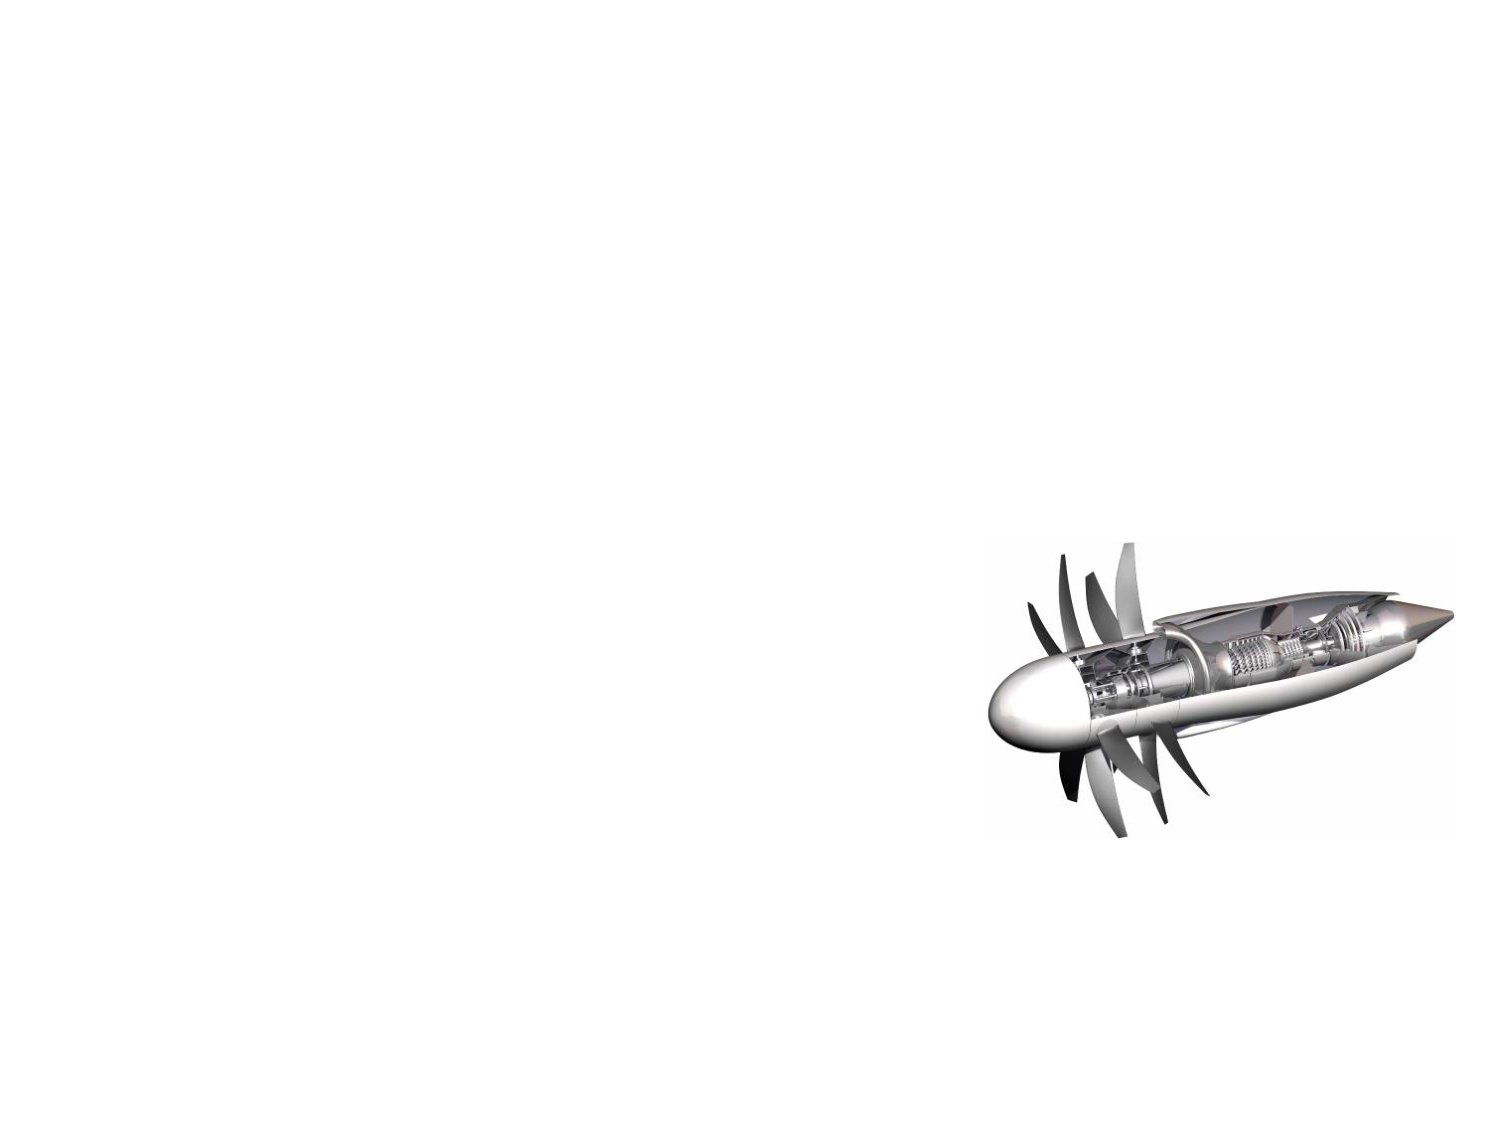
\includegraphics[width=0.45\textwidth]{puller.pdf}}
  \subfigure[pusher]{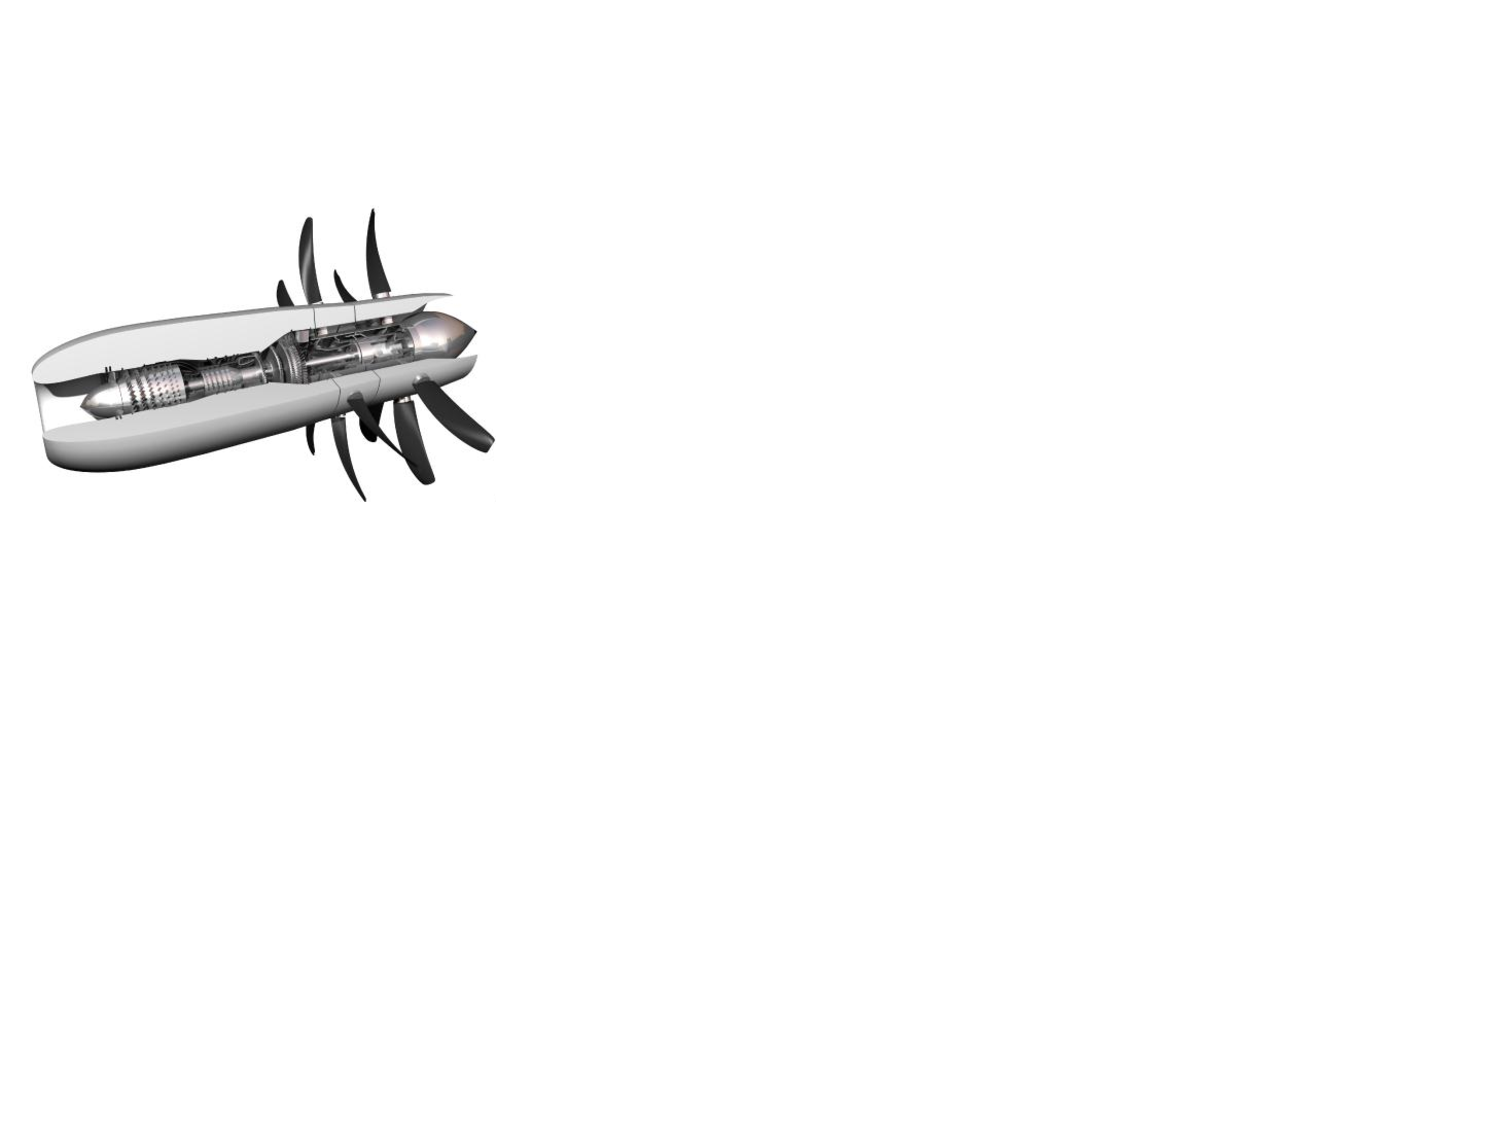
\includegraphics[width=0.45\textwidth]{pusher.pdf}}
  \caption{Types of contra-rotating open rotor, courtesy Rolls-Royce.}
  \label{fig:cror_configurations}
\end{figure}
% For pusher CROR, two types of architectures can be thought:
% one based on a gearbox and the second
% being build around a statorless low-pressure turbine. These
% two 
% \begin{figure}[htp]
%   \centering
%   \subfigure[geared design]{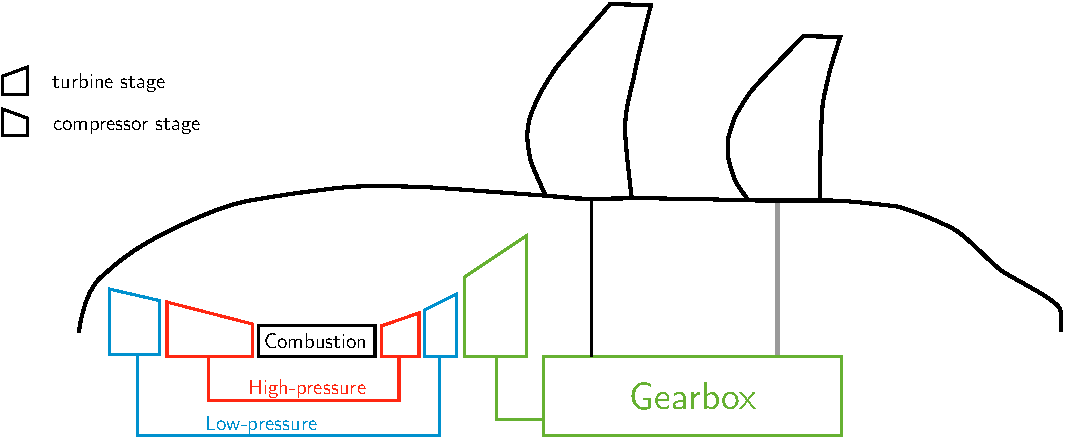
\includegraphics[width=0.45\textwidth]{geared_cror.pdf}}
%   \subfigure[statorless low-pressure turbine design]{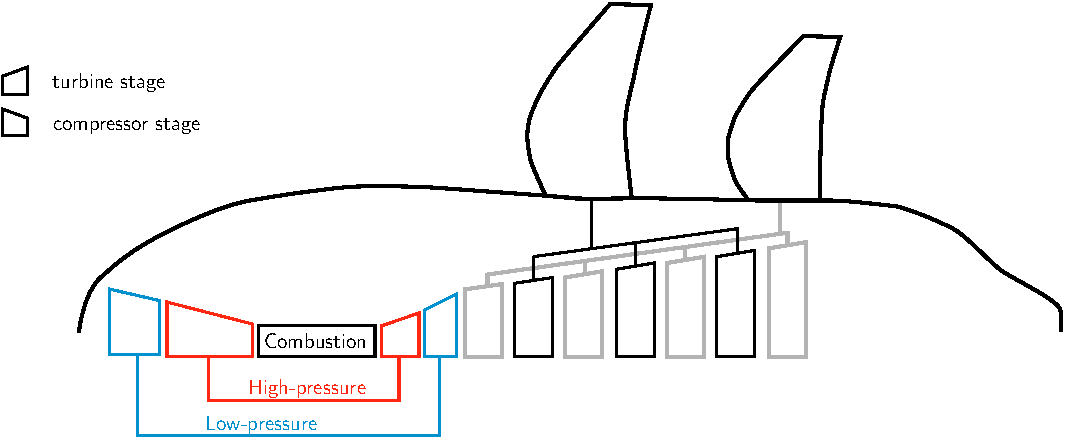
\includegraphics[width=0.45\textwidth]{stator_less_cror.pdf}}
%   \caption{Contra-rotating open rotor pusher architectures.}
%   \label{fig:cror_architectures}
% \end{figure}

\subsection{Velocity triangle}
\label{sub:cror_velocity_triangle}
\begin{figure}[htp]
  \centering
  \includegraphics*[scale=0.5]{velocity_triangle_cror.pdf}
  \caption{Velocity triangle applied to a contra-rotating open rotor.}
  \label{fig:velocity_triangle_cror}
\end{figure}
Figure~\ref{fig:velocity_triangle_cror} shows the application
of the velocity triangle to a CROR configuration. The swirl
energy that was lost by the propeller is now used to 
produce more thrust. Therefore, a CROR will finally have a better propulsive
efficiency than a propeller, which explains its study as
a greener engine. In the eighties, 
\citet{Strack1981} and \citet{Hager1988} showed that
using a contra-rotating open rotor technology over
a single propeller gave an increase of $6-8\%$
in propulsive efficiency, explaining its regain of interest.
Today, high-speed propellers blades might lead to higher increase
in efficiency
while keeping a flight Mach number close to $0.8$, enabling its use
for commercial aviation.

\subsection{Similarity coefficients}
\label{sub:cror_similarity_coeff}

In the case of a CROR configuration, the front and the rear rotors 
have to be considered.
Two main ways exist to evaluate the global value of the
similarity coefficients. The first one, chosen by
\citet{Bechet2011} among others, is to consider
that the non-dimensional parameter $D$, $n$ and $J$ are those
of the front rotor for both rotors
\begin{equation}
    J_f = J_r = \frac{V_0}{n_f D_f}, \quad
    C_T = \frac{F_{x_f} + F_{x_r}}{\rho_f n_f ^ 2  D_f ^ 4}, \quad
    C_P = \Omega_f \frac{M_{x_f} + M_{x_r}}{\rho_f n_f ^ 3 D_f ^ 5}, \quad
    \eta = J_f \frac{C_T}{C_P}.
\end{equation} 
The second one uses the non-dimensional parameter of the current rotor,
as done by \citet{Stuermer2008} and \citet{Zachariadis2011}.
The first approach is retained for the current work as it allows
to simplify the comparison of the similarity coefficient with equivalent propellers.


\section{Unsteadinesses}
\label{sec:cror_unsteady}
%!TEX root = ../../../adrien_gomar_phd.tex

\subsection{Unsteady effects}
\label{sub:cror_from_steady_to_unsteady_phenomena}

The flow field generated behind the front rotor
is steady in its frame of reference. Nevertheless,
due to the relative speed difference between the
front and the rear rotors, these steady flow distortions are
seen as unsteady features by the rear rotor. 
These unsteadinesses are correlated with the Blade Passing Frequency (BPF)
\begin{equation}
	f_{BPF} = \frac{\Omega_{rel} B_{opp}}{2 \pi},
\end{equation}
where $\Omega_{rel}$ is the relative speed difference between
the current and the opposite row
and $B_{opp}$ the number of blades in the opposite row.

\subsection{Main kinds of unsteadiness}
\label{sub:cror_main_unsteadinesses}

\paragraph{Wakes and potential effects}

Compared to an isolated rotor, as for the case of a propeller,
the presence of the rear rotor gives rise to an unsteady
interaction by means of potential effects. In addition, wakes generated
behind the front rotor interact with the rear rotor.
This is schematically represented in Figure~\ref{fig:cror_wakes_potential}.
\begin{figure}[htp]
  \centering
  \includegraphics*[width=0.4\textwidth]{cror_wakes_potential.pdf}
  \caption{Wakes and potential effects in a 
  contra-rotating open rotor.}
  \label{fig:cror_wakes_potential}
\end{figure}
These two phenomena are correlated with the blade passing frequency.
In addition to this, vortex shedding phenomena may occur behind the blades, 
the frequency of which is not known \emph{a priori}.
This phenomenon is more likely to appear behind blades with a bluff trailing edge.
However, this is not a common design for industrial compressor 
configurations as bluff trailing edges
give larger drag. Therefore, we can consider here that 
wake and potential effects are the main unsteady phenomena,
and these are correlated with the blade passing frequency.

\paragraph{Non-uniform inflow and installation effects}

In maneuver, the CROR is in incidence with respect to the incoming flow
which results in a non-uniform velocity triangle on the blades.
This leads to in-plane forces, which represents an unsteady phenomenon
whose frequency is correlated with the rotation frequency $\Omega / 2 \pi$.
The presence of a pylon (installation effect) gives rise to an unsteady frequency
also correlated with the rotation frequency when a pusher CROR is considered.
It is important as it changes both performance and flow behavior around the CROR.


\section{Challenges}
\label{sec:cror_challenges}
%!TEX root = ../../../adrien_gomar_phd.tex

Several challenges are still open for CROR
to become a viable engine for the next generation aircraft.
In this way, we classify and describe each of them in the following sections.

\paragraph{Classification}
Figure~\ref{fig:cror_challenges} depicts current challenges associated
with CROR configurations. Three main fields are involved: Aerodynamics,
Aeroacoustics and Aeroelasticity.
\begin{figure}[htp]
  \centering
  \includegraphics*[scale=0.8]{challenges.pdf}
  \caption{Challenges raised by contra-rotating open rotors.}
  \label{fig:cror_challenges}
\end{figure}

\paragraph{Aerodynamics}
Theoretically, 
the CROR is meant to have a better propulsive efficiency than a turbofan or a
propeller. However, as it is a new architecture, studies need to be conducted
to better understand the inherent flow physics. In particular,
aerodynamic interactions between the two rotors need to be better understood.

Research on the Aerodynamics of CROR is divided in two main
axes: the first axis deals with the design of CROR while the second
one analyzes the unsteady flow physics that develop on a given design.

Concerning the first axis, 
\citet{Hendricks2011} developed an open-rotor cycle model based
on experimental performance characteristics made at NASA. This is 
an empiric approach that suffers from the impossibility to build new designs.
\citet{Peters2012} developed a similar code to design their CROR. The aeroacoustic
characteristics of the final design is assessed by a 
full annulus unsteady simulation even though the design is 
based on experimental correlations.
To improve the approach to design new CROR, 
\citet{Bechet2011} used a lifting-line code to
initialize a gradient optimization procedure based on mixing-plane
computations. This led to a gain of almost a half point
in CROR efficiency. This is more general than an empiric strategy
if the mixing-plane computations are reliable to assess the performance
parameters of CROR. 

Concerning the second axis, \citet{Zachariadis2011}
compared the performance prediction of mixing plane computations
to experimental data made on an open-rotor test case.
They found a fair agreement for the thrust and power coefficients, however
small discrepancies on the coefficients led to significant errors on their ratio,
\emph{i.e.} the efficiency.
\citet{Vion2011} and \citet{Stuermer2008} used unsteady
CFD computations to assess the unsteady performance and flow features.
\citet{Stuermer2008} and \citet{Francois2013} demonstrated through a code to code comparison
that CFD was mature enough to estimate in-plane forces.

\paragraph{Aeroacoustics}
Lot of research efforts are put on the second challenge which
is Aeroacoustics since the absence of a duct allows noise generated
by CROR to propagate far away.
In the late eighties, \citet{Hager1988}
conducted at NASA a large project on innovative propulsion systems for the
next generation aircrafts. The potential of the CROR configuration
was identified but the noise emitted was so high that the only way
thought to use such an engine was to put noise liners in the fuselage. This resulted in 
increased weight. This is why, today, a lot of research effort is put on the
understanding and mastering of noise sources in CROR.
Two main types of noise have been identified: tonal noise which comes from
the interaction of both rotors and is mainly present at low-speed flight conditions 
(namely take-off and landing)
and broadband noise which comes from turbulence and is predominant
at high-speed flight conditions (namely cruise).
Several CFD studies have been performed in the literature.
\citet{Peters2012} showed that unsteady CFD simulation is able
to reproduce the aeroacoustic footprint of a CROR. They then optimized
their CROR and showed that this optimized CROR design may be mature enough
for noise certification. \citet{Hoffer2012} and \citet{Ferrante2013}
developed an efficient CFD approach to simulate the aeroacoustics of CROR.
It is based on a Fourier-based time method. The approach is able to
account for incidence effects which is particularly interesting
considering that the noise of installed configuration is drastically
different from the isolated one (see \citet{Hager1988}).

\paragraph{Aeroelasticity}
The third challenge is less studied in the numerical literature.
Three main aeroelastic phenomena have been identified during preliminary studies
during the eighties by \citet{Hager1988}: whirl flutter, \emph{i.e.} the self-excited
movement of the whole nacelle, blade flutter, \emph{i.e.} the vibration
of the blades, and forced response, \emph{i.e.} the excitation of blades modes
by the distortions shed by the rotors or the pylon.
For a turbofan engine to achieve certification, it must be 
demonstrated that one released fan blade can be safely contained 
within the engine’s fan case as written in the 
Certification Specifications for Engines (CSE) of the EASA:
\begin{quote}
	"It must be demonstrated that any single compressor or turbine blade will be contained after Failure and 
that no Hazardous Engine Effect can arise as a result of other Engine damage likely to occur before 
Engine shut down following a blade Failure"
\end{quote}
In the case of propellers and contra-rotating open rotors, due to the absence of a nacelle,
this can not be done. To achieve certification, it must be demonstrated that the probability of a blade
failure (or any failure) should not exceed $10^{-8}$ per propeller flight hour as written in 
the Certification Specifications for Propellers (CSP) of the EASA:
\begin{quote}
	"It must be shown that Hazardous Propeller Effects will not occur at a rate in excess of that defined 
as Extremely Remote. The estimated probability for individual failures may be insufficiently precise 
to enable the total rate for Hazardous Propeller Effects to be assessed. For Propeller certification, it 
is acceptable to consider that the intent of this paragraph is achieved if the probability of a 
Hazardous Propeller Effect arising from an individual failure can be predicted to be not greater than 
$10^{-8}$ per Propeller flight hour. It will also be accepted that, in dealing with probabilities of this low 
order of magnitude, absolute proof is not possible and reliance must be placed on engineering 
judgment and previous experience combined with sound design and test philosophies" 
\end{quote}
This explains why aeroelasticity of contra-rotating open rotors should be assessed.
Whirl flutter and forced response have been investigated
in the CROR literature. The former has been assessed by \citet{CISicot2011a} and 
\citet{Verley2013} but these studies mainly
discuss the simulation tools needed to compute such a phenomenon as
no experimental data are available.
The latter has been investigated by \citet{Ruiz-Calavera2012}
on installed puller propellers and by \citet{Laban2010} on
CROR using a strong-coupling approach. 



\chconclu{The concept of contra-rotating open rotor has
been presented along with the basic flow phenomena that develop within it.
These unsteady phenomena are mostly 
correlated with the blade passing frequency, except for
the installation effects and the non-uniform inflow. The challenges
associated with this type of engine are recalled and it is highlighted 
that aeroelasticity of such systems remain to be accounted for. This is
why the present work will focus on aeroelasticity, which is
introduced in the following chapter.}
